\documentclass[border=10pt]{standalone}

\usepackage{tikz}
\usepackage{tikzsymbols}
\usetikzlibrary{calc,patterns,shapes.geometric}

\def\centerarc[#1](#2)(#3:#4:#5){\draw[#1] ($(#2)+({#5*cos(#3)},{#5*sin(#3)})$) arc (#3:#4:#5);}

\begin{document}
	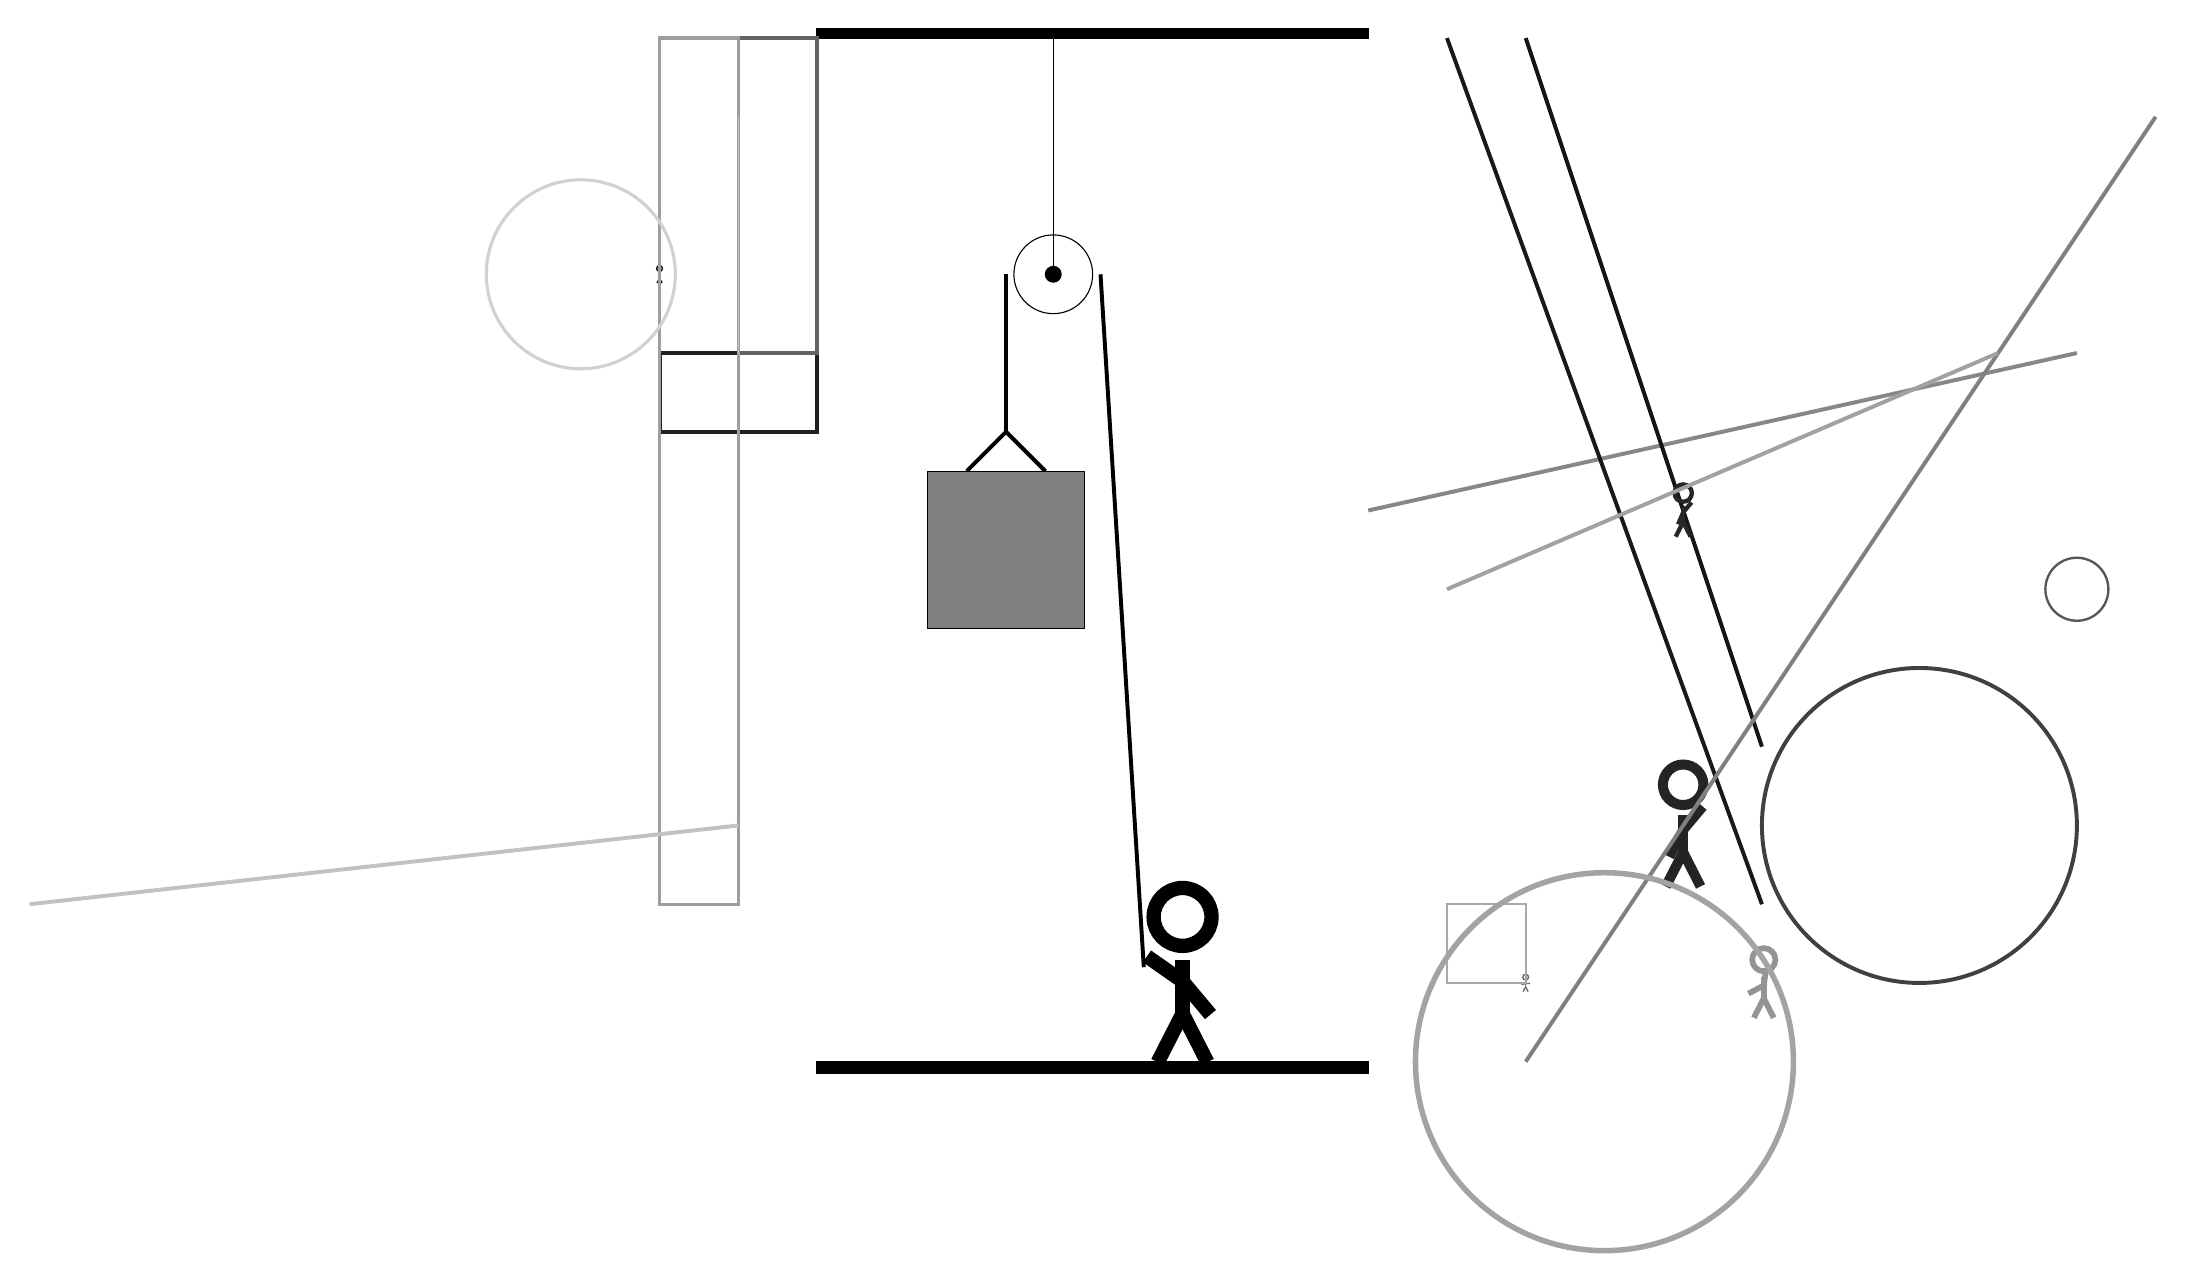
\begin{tikzpicture}
		%%%%% START %%%%%
		
		\draw[fill=black] (-2, 10) rectangle (5, 10.125);
		
		\draw[line width=0.5mm, color=black!47](5, 4) -- (14, 6);
		
		\draw[line width=0.5mm, color=black!90](10, -1) -- (6, 10);
		\draw[line width=0.5mm, color=black!92](7, 10) -- (10, 1);
		\node[line width=0.2mm, color=black!85] at (9, 4) {\Strichmaxerl[3][67][50]};
		\node[line width=0.3mm, color=black!93] at (-4, 7) {\Strichmaxerl[1][88][77]};
		
		\node[line width=0.5mm, color=black!86] at (9, 0) {\Strichmaxerl[7][63][50]};
		\draw[line width=0.5mm, color=black!87] (-4, 5) rectangle (-2, 6);
		
		\node[line width=0.2mm, color=black!42] at (10, -2) {\Strichmaxerl[4][28][82]};
		\draw[line width=0.5mm, color=black!50](7, -3) -- (15, 9);
		\draw[line width=0.4mm, color=black!61] (-3, 10) rectangle (-2, 6);
		\node[line width=0.2mm, color=black!57] at (7, -2) {\Strichmaxerl[1][11][2]};
		\draw[line width=0.3mm, color=black!34] (7, -2) rectangle (6, -1);
		\draw[line width=0.4mm, color=black!38] (-3, 10) rectangle (-4, -1);
		\draw[line width=0.2mm, color=black!25] (-3, 6) rectangle (-3, 9);
		\draw[line width=0.5mm, color=black!24](-3, 0) -- (-12, -1);
		\draw [line width=0.4mm, color=black!18](-5, 7) circle (1.2);
		
		\draw [line width=0.7mm, color=black!36](8, -3) circle (2.4);
		\draw[line width=0.5mm, color=black!37](6, 3) -- (13, 6);
		\draw [line width=0.3mm, color=black!66](14, 3) circle (0.4);
		
		\draw [line width=0.5mm, color=black!75](12, 0) circle (2.0);
		
		\draw (1, 7) circle (0.5);
		\draw[fill=black] (1, 7) circle (0.1);
		\draw (1, 10) -- (1, 7);
		
		\draw[line width=0.5mm] (-0.1, 4.5) -- (0.4, 5.0) -- (0.9, 4.5);
		\draw[fill=black!50] (-0.6, 4.5) rectangle (1.4, 2.5);
		
		\draw[line width=0.5mm] (0.4, 7) -- (0.4, 5.0);
		\centerarc[line width=0.5mm](1, 7)(0:180:0.6);
		\draw[line width=0.5mm](1.6, 7) -- (2.15, -1.8);
		
		\node at (2.6, -1.9) {\Strichmaxerl[10][-35][-50]};
		
		\draw[fill=black] (-2, -3) rectangle (5, -3.15);
		
		%%%%% END %%%%%
	\end{tikzpicture}
\end{document}